
\documentclass[letterpaper, 11pt]{article}
\usepackage{titlesec}
\usepackage{fullpage} % changes the margin
\usepackage{amsmath}
\usepackage{amssymb}
\usepackage{graphicx} %package to manage images
\usepackage{paralist}
\usepackage{subcaption}
\graphicspath{ {./images/} }

\begin{document}
\begin{titlepage}
\vspace*{0.7in}
\begin{center}
\begin{figure}[htb]
\begin{center}

\includegraphics[width=8cm]{univ_logo}
\end{center}
\end{figure}
\vspace*{0.3in}
\begin{Large}
\textbf{SOEN 6011 : SOFTWARE ENGINEERING PROCESSES} \\
\end{Large}
\vspace*{0.1in}
\begin{Large}
\textbf{SUMMER 2022} \\
\end{Large}
\vspace*{0.9in}
\begin{Large}
\textbf{ETERNITY} \\
\end{Large}
\vspace*{0.625in}
\begin{Large} 


\textbf{PROBLEM - 1} \\
\vspace*{0.2in}
Function Description\\
\vspace*{0.1in}
\end{Large}
\vspace*{0.625in}
\rule{80mm}{0.1mm}\\
\vspace*{0.1in}
\begin{large}
Author \\
\vspace*{0.1in}
Neona Sheetal Pinto\\
\vspace*{1.0in}
\date{\normalsize\today} 
\end{large}
\end{center}
\begin{center}
https://www.overleaf.com/project/62e93df32b39377e64b9456e\end{center}
\end{titlepage}



\tableofcontents
\listoffigures
\newpage
\section{PROBLEM 1 - F6: $B(x,y)$}
    \subsection{Description -  Beta Function, $B(x,y)$ } 
         \normalsize{ \cite{mathworld} $B(x,y)$ The beta function (also known as Euler's integral of the first kind) is important in calculus and analysis due to its close connection to the gamma function, which is itself a generalization of the factorial function. Many complex integrals can be reduced to expressions involving the beta function, for inputs such that $x, y > 0$. This is a proportional function like B(x, y) = B(y, x) and this is a special mathematical function. This special type of function of mathematics, the Beta function, was invented by the Swiss mathematician Leonhard Euler and the graph for Beta function can be shown in figure \ref{fig:beta_graph} \cite{mathworld}\cite{byjus}\\
                            
        \begin{center}
            ${B}(x,y)=\int _{0}^{1}t^{x-1}(1-t)^{y-1}\,dt$ 
        \end{center}
         }
 
    \subsection{Graph}
        \begin{figure}[htb]
            \begin{center}
                  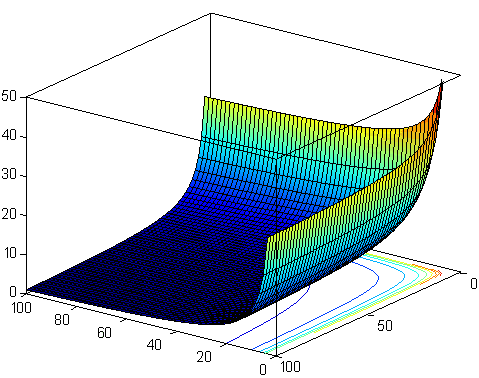
\includegraphics[width= 7cm]{images/BetaFunction.png}
            \end{center}
             \caption{ Graph of Beta function on real plane $B(x,y)$}
            \label{fig:beta_graph}
        \end{figure}


    \subsection{Domain and Co-domain}
         \normalsize{
         A domain is the set of values that behaves as input in the function while it can be defined. Beta Function is specified in real-number domains or complex number inputs $z_{1},z_{2}$  such that ${\qquad \Re (z_{1}),\Re (z_{2})>0\ }$ \\
         The co-domain is also the same as above, ${\Re (z_{1}),\Re (z_{2})>0\ }$
         }\cite{collegedunia}\cite{wiki}
    \subsection{Range}\cite{wiki}
        \normalsize{ The range of $B(x,y)$ is all real number $\mathbb{R}$, $(0, + \infty)$. }
\pagebreak
    \subsection{Context of Use Model}
        \normalsize{The users of the Eternity shall be using it to calculate the result of Beta functions on values x and y. This number shall be an integer or decimal, so the digits \textit{0-9} and the decimal point must be entered by the user if they wish to do so. The values have to be positive. The user shall be able to select the appropriate options displayed in the command line interface they wish to use, and they shall be able to perform the operation to indicate that they have finished inputting the number and wish to have the answer computed. The calculator should return the result. In case of wrong inputs a message that indicates why it was unable to do so should be displayed. The user can also opt to get more information on the Beta function if they wish to read about it. The user can quit if they wish to stop. The context of use of Eternity is shown in the above figure \ref{fig:context}}.
        
        \begin{figure}[htb]
            \begin{center}
                  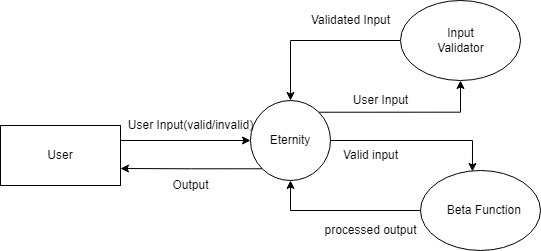
\includegraphics[width= 15cm]{images/context_diagram.png}
            \end{center}
             \caption{ Context Use of Eternity Model}
            \label{fig:context}
        \end{figure}
        
\newpage
\section*{Annexure:}
    \begin{itemize}
      \item \textbf{Trello Board :} \textit{https://trello.com/eternity119}
      \item \textbf{Code Version Control :} \textit{https://github.com/neonapinto/Scientific\_calculator}
      \item \textbf{Overleaf :} \textit{https://www.overleaf.com/project/62e93df32b39377e64b9456e}
    \end{itemize}
    
\begin{thebibliography}{}
     
    \bibitem{mathworld}
    https://mathworld.wolfram.com/BetaFunction.html
    
    \bibitem{byjus} 
    https://byjus.com/maths/beta-function
    
    \bibitem{collegedunia} 
    https://collegedunia.com/exams/beta-function-definition-properties-formula-and-examples-mathematics-articleid-5443
    
    \bibitem{wiki} 
    https://en.wikipedia.org/wiki/Beta\_function
\end{thebibliography}

\end{document}
